\section*{Appendix}

\subsection*{Hyperparameters}
We use the Deepmind Lab environment to train our experiments. 
As mentioned previously, apple rewards are scattered throughout the maze and constitute a +1 reward. 
Goals constitute a +10 reward. An included wall penalty linearly penalizes the agent as it moves closer to the wall with the penalty being capped off at -.2 per frame.
Our episodes are of fixed time length ending at 40 seconds each.
The agent interacts with the environment at a rate of 30 frames per second. 
Each episode thus consists of 1200 frames of data coupled with the corresponding reward signals.
Our mazes constitute an area of $900 units \times 900 units$ though we provide the tools to generate mazes to arbitrary dimensions. 

Our A3C implementation is a modified version of OpenAIs open-sourced \emph{universe-starter-agent}. RGB images are fed in to the network of dimensions $84\times84\times3$. 16 threaded agents are used for all experiments. We use a learning rate of $10^{-4}$ along with the \emph{AdamOptimizer} to train our network. Our models train for a maximum of $10^{8}$ iterations though we end them early if maximum reward saturates. 

\subsection*{Benchmarking code}
To motivate more comprehensive experimental evaluations of DRL-based navigation methods, we will be releasing all our trained models coupled with corresponding reward curves and videos of performance online. 
This will include completely reproducible evaluation sets wherein we display metric scores for all the trained models on the follow environments:
\begin{itemize}
    \item the original training conditions
    \item the training conditions in the absence of apples and textures
    \item the 100 unseen testing maps
    \item the planning maps i.e. the square, wrench and goal map
\end{itemize}
We hope our work can also be utilized as a stepping stone for the creation of better generalized DRL navigation methods bypassing the needless amounts of time spent engineering the infrastructure necessary for these experiments. 
All our work will be available on github after the blind-review process is over.

\subsection{Reward curves with different number of training maps}
\begin{figure}[h]%
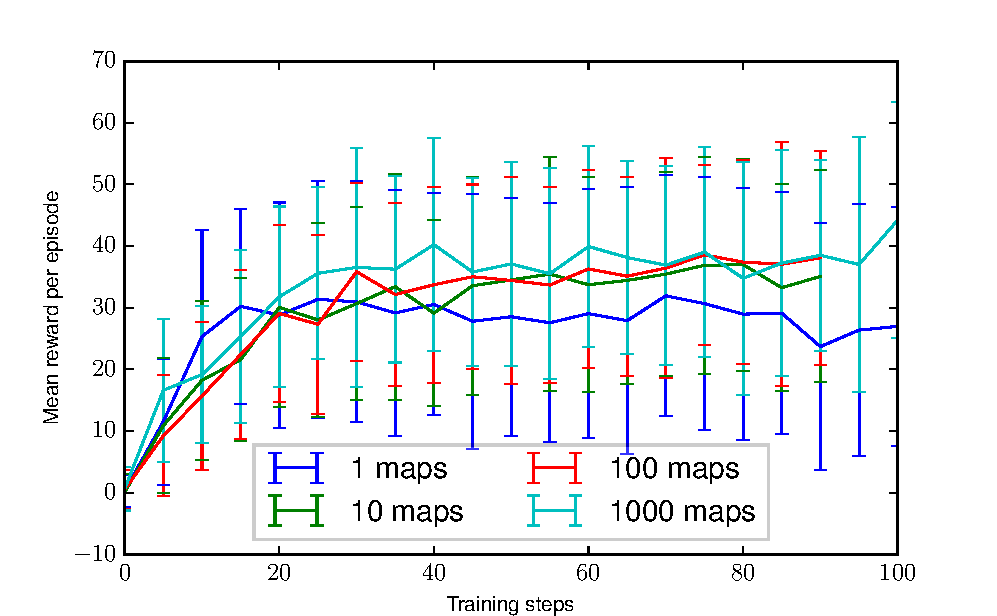
\includegraphics[width=0.5\columnwidth]{images/plot_reward_3D-1000.pdf}%
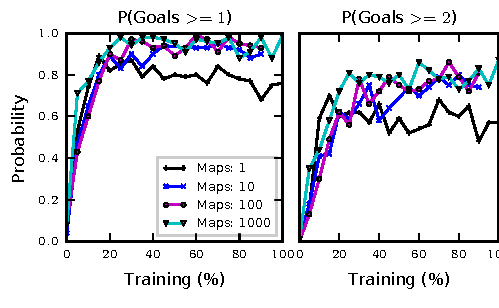
\includegraphics[width=0.5\columnwidth]{images/plot_probability_3D-1000.pdf}%
\vspace{-1em}%
\caption{Mean reward while tested on 100 unseen maps, while being trained on different number of training maps. Note that while training on 1000 maps eventually achieves high reward, it is only higher mean reward (44.2), training on 1 map hits the maximum (31) much faster.}%
\label{fig:plot_reward_on_testing}%
\end{figure}

